\section{Simulation Validation}
\label{appendix:simulation_validation}

\noindent\textit{This appendix validates that the two dynamics models used by
controllers in the main paper, the analytical first-principles model and the
learned LSTM world model, are accurate enough predictors of real hardware
dynamics.  Rather than comparing controller-level metrics (success rate,
settling time), we evaluate open-loop trajectory prediction accuracy against
held-out partitions of the 1\,M-transition real dataset.  This isolates model error from
controller behavior and provides a direct measure of simulation fidelity.}

\subsection{Methodology}
\label{sec:sim_val_method}

We follow a standard open-loop prediction protocol:
\begin{enumerate}
  \item From a dataset of real hardware transitions
        $(\mathbf{s}_t, a_t, \mathbf{s}_{t+1})$, select $N$ reset-free
        segments of length $L$.
  \item For each segment, initialize a candidate model to the real state
        $\mathbf{s}_0$ and replay the recorded action sequence
        $a_0, a_1, \dots, a_{L-1}$ open-loop.
  \item Record the predicted trajectory
        $\hat{\mathbf{s}}_1, \dots, \hat{\mathbf{s}}_L$ and compute
        terminal MAE $|\hat{\mathbf{s}}_L - \mathbf{s}_L|$ and
        trajectory MAE $\frac{1}{L}\sum_{t=1}^{L} |\hat{\mathbf{s}}_t - \mathbf{s}_t|$.
  \item Report means across all segments.
\end{enumerate}

\paragraph{Metric choice.}
We report mean absolute error (MAE) rather than root-mean-square error (RMSE)
because MAE is robust to outliers and directly interpretable in physical units.
Since the four state variables operate on very different scales (cart position
$\pm 0.78$\,m, ball angle $\pm 0.081$\,rad), we also report \emph{normalized MAE}
(MAE divided by the variable's full operating range, expressed as a percentage).
Normalized MAE makes channels comparable and reveals which state dimensions
are predicted most poorly relative to their dynamics.

We use two configurations:
\begin{itemize}
  \item \textbf{Exp 1 (short horizon):} $N=100$ segments, filtered to
        initial conditions (IC) with $|\theta| < 0.04$\,rad
        (ball near center), horizons $0.25$--$2.5$\,s ($5$--$50$ steps).
        This corresponds to the prediction horizon used by model-based
        controllers (MPPI, NMPC).
  \item \textbf{Exp 2 (long horizon):} $N=50$ segments with no IC filter,
        horizons $0.25$--$30$\,s ($5$--$600$ steps).
        This covers the episode length used by RL agents.
\end{itemize}

Under the 80/10/10 split used to train the world model, the analytical
ablation (Exp 1, which selects the best analytical configuration) draws
segments from the validation partition (rows 80--90\%), and the
world-model comparison (Exp 2) draws from the held-out test partition
(rows 90--100\%). Neither partition receives gradient updates; the
validation partition (Exp 1) is used only for early stopping and
checkpoint selection, while the test partition (Exp 2) is fully held out
and drives the primary world-model comparison. Both slices are disjoint
from the one used to pick the analytical configuration.

The candidate models are:
\begin{itemize}
  \item \textbf{Analytical model}: the velocity-input first-principles model
        (Section~\ref{sec:velocity_input}) with nominal parameters
        ($\tau_v = 0.15$\,s, $d = 0.002$\,m, $\mu_\mathrm{rr} = 0.025$,
        $\beta_v = 0.009$~m$^2$/s), Euler integration with step size
        0.05\,s, a 1-step command delay, and a first-order velocity
        observation filter (PT1, $\tau = 10$~ms).
        Additional structural variants are compared in the ablation below.
  \item \textbf{World model}: a 2-layer LSTM (hidden dim~64, sequence
        length~10) trained on 1\,M real transitions, as detailed in
        Appendix~\ref{appendix:world_model}.  It predicts the state delta
        $\Delta\mathbf{s}_{t+1}$ with a skip connection.  During rollout
        the LSTM hidden state is maintained across steps to capture
        temporal dynamics.
\end{itemize}

\subsection{Analytical Model Ablation}
\label{sec:sim_val_ablation}

Before comparing against the world model, we ablate the analytical model
to quantify the contribution of each pipeline component.  All ablations
are at $h=50$ ($2.5$\,s).

\paragraph{Pipeline components.}
Figure~\ref{fig:sim_val_waterfall_pipeline} shows the cumulative effect
of adding each pipeline element.  The bare model ($\tau_v = 0.06$, no
delay, no filter) has a total trajectory MAE (sum over 4 channels)
of 0.756.  Calibrating $\tau_v$ to 0.15 reduces this to 0.521, a 31\%
improvement that accounts for the majority of the total gain.  Adding
a discrete one-step (50\,ms) command-delay approximation
further reduces error to 0.476. The 50\,ms one-step delay is a
conservative upper bound on the measured real transport delay (under
14\,ms) and is retained in the training and tuning simulators
(Appendices~\ref{appendix:rl_training} and~\ref{appendix:tuning_insights}).  The velocity observation filter (PT1,
$\tau = 10$\,ms) adds a small additional improvement to 0.444.

\begin{figure}[!tbp]
  \centering
  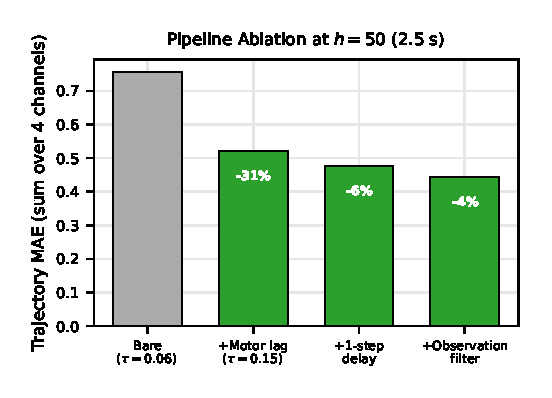
\includegraphics[width=\columnwidth]{figures/sim_val_waterfall_pipeline.eps}
  \caption{Pipeline ablation: total trajectory MAE (sum of 4 channels)
           at $h=50$ ($2.5$\,s).  Calibrating $\tau_v$ accounts for the
           largest improvement; command delay and observation filtering
           provide diminishing returns.}
  \label{fig:sim_val_waterfall_pipeline}
\end{figure}

The normalized MAE (Table~\ref{tab:sim_val_ablation}) shows that ball
angle $\theta$ has the highest relative error (33\% of operating range
even with the bare model), confirming that the ball dynamics are the
hardest channel to predict regardless of modeling choices.

\begin{table*}[!t]
\centering
\caption{Pipeline ablation: normalized trajectory MAE (\% of operating range)
         at $h=50$ ($2.5$\,s).  Raw MAE values in parentheses.}
\label{tab:sim_val_ablation}
\begin{tabular}{lcccc}
\toprule
Variant & $x$ & $\dot{x}$ & $\theta$ & $\dot{\theta}$ \\
\midrule
Bare ($\tau_v = 0.06$)
  & 6\%\,(0.099)  & 23\%\,(0.417)  & 33\%\,(0.054) & 19\%\,(0.186) \\
$+\tau_v = 0.15$
  & 5\%\,(0.084)  & 15\%\,(0.267)  & 28\%\,(0.046) & 12\%\,(0.124) \\
$+$Delay (1 step)
  & 5\%\,(0.082)  & 13\%\,(0.226)  & 30\%\,(0.048) & 12\%\,(0.120) \\
$+$Obs filter
  & 5\%\,(0.082)  & 12\%\,(0.208)  & 29\%\,(0.047) & 11\%\,(0.108) \\
\bottomrule
\end{tabular}
\end{table*}

\paragraph{Best analytical configuration.}
Based on this ablation, the best analytical model is: velocity-input
first-principles ball dynamics, first-order velocity lag
($\tau_v = 0.15$\,s), 1-step command delay, and velocity observation
filter (PT1, $\tau = 10$\,ms).  This configuration is used as the
``analytical model'' in the remainder of this appendix and in all
controllers that rely on the analytical simulator.

\subsection{Analytical Model vs.~World Model}
\label{sec:sim_val_comparison}

We now compare the best analytical model against the LSTM world model.
Table~\ref{tab:sim_val_comparison} reports terminal MAE as a percentage
of each channel's operating range.

\begin{table*}[!t]
\centering
\caption{Terminal MAE (\% of operating range) at representative horizons.
         Negative $\Delta$ indicates world model improvement.}
\label{tab:sim_val_comparison}
\begin{tabular}{llccccc}
\toprule
Horizon & Model & $x$ (\%) & $\dot{x}$ (\%) & $\theta$ (\%) & $\dot{\theta}$ (\%) & Avg. (\%) \\
\midrule
\multirow{3}{*}{0.25\,s}
  & Analytical  & 2 & 13 & 11 & 11 & 9 \\
  & World Model & 2 &  9 &  7 &  5 & 6 \\
  & $\Delta$    & $+4$\% & $-34$\% & $-34$\% & $-55$\% & \\
\addlinespace
\multirow{3}{*}{2.5\,s}
  & Analytical  & 8 & 12 & 31 & 10 & 15 \\
  & World Model & 9 &  7 & 40 &  6 & 16 \\
  & $\Delta$    & $+2$\% & $-46$\% & $+30$\% & $-37$\% & \\
\addlinespace
\multirow{3}{*}{10.0\,s}
  & Analytical  & 11 & 15 & 38 & 12 & 19 \\
  & World Model & 10 &  5 & 36 &  7 & 15 \\
  & $\Delta$    & $-10$\% & $-70$\% & $-6$\% & $-45$\% & \\
\addlinespace
\multirow{3}{*}{30.0\,s}
  & Analytical  & 20 & 14 & 42 &  8 & 21 \\
  & World Model & 15 &  4 & 42 &  8 & 17 \\
  & $\Delta$    & $-28$\% & $-70$\% & $-1$\% & $+8$\% & \\
\bottomrule
\end{tabular}
\end{table*}

Figure~\ref{fig:sim_val_error_growth} visualizes the full error growth
curves.

\begin{figure*}[!tbp]
  \centering
  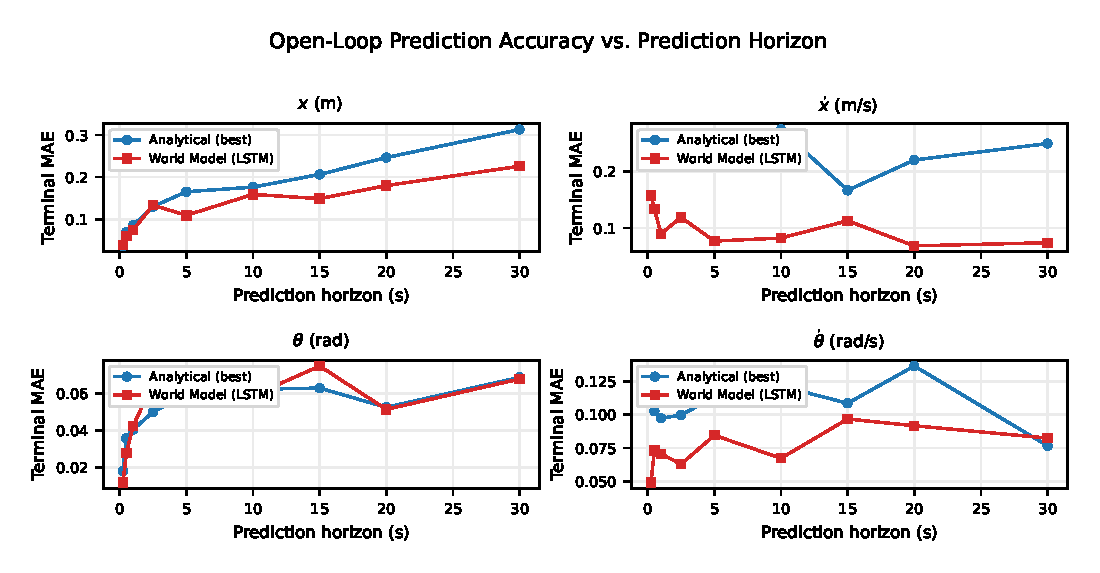
\includegraphics[width=\textwidth]{figures/sim_val_error_growth.eps}
  \caption{Terminal MAE vs.~prediction horizon for the analytical model
           (blue) and world model (red), one panel per state channel.
           The world model has lower terminal MAE at most horizons on cart
           position and both velocities; the exception is terminal ball-angle
           error, where the analytical model matches or beats it at 1, 2.5,
           5, and 15\,s.
           Error growth is sub-linear for both models,
           indicating no catastrophic divergence.}
  \label{fig:sim_val_error_growth}
\end{figure*}

\paragraph{Normalized perspective.}
Normalized MAE reveals that the analytical model's weakest channel is
ball angle $\theta$: at 2.5\,s it reaches 31\% of the ball's total
range, and at 30\,s it reaches 42\%.  Cart position and velocity stay
below about 20\% even at the longest horizon.  This asymmetry reflects the
indirect coupling: $\theta$ is driven through the arc geometry, which
amplifies residual error from the cart model.

The world model's advantage is largest on cart velocity
($\dot{x}$ improves by 34--70\% across the horizons). For ball angle
$\theta$ the two models are close, and the world model is actually worse
at 2.5\,s ($+30$\%). This is because ball angle is primarily determined by the
physical geometry and gravity, dynamics that both models capture
equally well, while velocity dynamics are more sensitive to the
unmodeled servo behavior that the LSTM learns.

\subsection{Crossover Analysis}
\label{sec:sim_val_crossover}

A key question is whether there exists a prediction horizon at which
the simpler analytical model matches or beats the learned world model,
i.e., a \emph{crossover}.  Figure~\ref{fig:sim_val_crossover} shows
the ratio of world model to analytical total trajectory MAE across
all horizons.

\begin{figure}[!tbp]
  \centering
  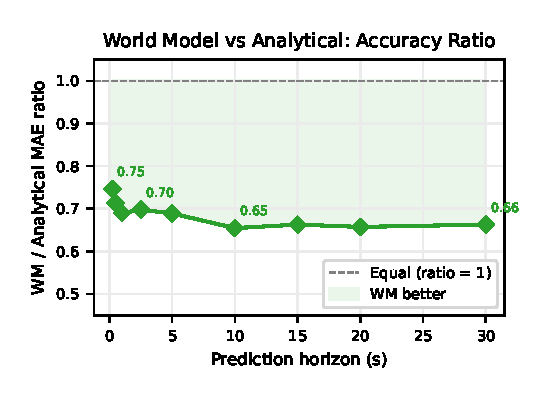
\includegraphics[width=\columnwidth]{figures/sim_val_crossover_ratio.eps}
  \caption{Ratio of world model to analytical total MAE vs.~prediction
           horizon.  Values below~1 indicate the world model is more
           accurate.  The world model wins at every horizon on total error; no crossover
           exists.  The ratio stays between about 0.65 and 0.75
           (25--35\% lower error), with the smallest margin at 0.25\,s and
           the largest around 10\,s.}
  \label{fig:sim_val_crossover}
\end{figure}

\paragraph{Crossover across horizons.}
The world model has lower total trajectory MAE across all tested
horizons ($0.25$--$30$\,s), by between 25 and 35\%: it is 25\% lower at
0.25\,s, peaks near 35\% around 10\,s, and holds about 34\% out to 30\,s.
There is no regime where the analytical model catches up on total error. These are point estimates from a single
evaluation run (100 segments in Exp 1, 50 in Exp 2); per-segment
dispersion, confidence intervals, and paired significance tests are not
reported, so the ordering is descriptive rather than statistically tested.

\paragraph{Implication for controller selection.}
For sampling-based predictive controllers that roll out many candidate
trajectories through the model (e.g.~MPPI with $H = 30$, a 1.5\,s
lookahead), the world model provides the largest relative benefit,
because every sampled trajectory inherits the model's higher fidelity
over the full rollout.  For classical and predictive controllers designed
around the analytical model (LQR+WO, MPC+WO, NMPC, SMC+WO), the analytical
model is sufficient: its short-horizon accuracy (0.018\,rad at
0.25\,s, 11\% of range) is adequate for feedback correction, and
closed-loop control compensates for residual model error.
For model-free RL trained purely in simulation (PPO~(BZ+DR), SAC~(DR),
TD3~(DR), TQC~(DR), TRPO~(DR)), the analytical model is likewise
sufficient because domain randomization and the controller's own
robustness absorb the
prediction gap, as confirmed by the hardware success rates in the
main paper.

The world model provides its largest benefit in two settings: (i)~zero-shot
deployment of PPO-WM, which achieves 100\% hardware success rate without
domain randomization, and (ii)~real-time trajectory optimization in MPPI,
where the learned model's higher fidelity directly improves sampled
trajectory quality relative to the analytical model.

\subsection{Summary}

\begin{enumerate}
  \item \textbf{Pipeline components contribute unequally.} Calibrating
        $\tau_v$ accounts for the largest improvement.  Command delay
        and observation filtering provide diminishing returns.
  \item \textbf{Ball angle is the hardest channel.} Normalized MAE for
        $\theta$ reaches 31\% of range at 2.5\,s (analytical model),
        compared to 8--12\% for the other channels.
  \item \textbf{World model has lower trajectory-mean error.} Its total
        trajectory MAE is 25--35\% lower than the analytical model's at
        every horizon (the analytical model is about 1.3--1.5$\times$
        higher), with the largest advantage on cart velocity ($\dot{x}$).
        Terminal ball-angle error is mixed: the analytical model matches
        or beats the world model at 1, 2.5, 5, and 15\,s.
  \item \textbf{Analytical model is sufficient for its use cases.}
        Classical, predictive, and domain-randomized RL controllers reach
        high hardware success with the analytical model, which suggests
        closed-loop feedback and domain randomization absorb the residual
        prediction error. This is an inference from open-loop prediction
        accuracy and the measured hardware success rates, not a controlled
        controller-level swap of the dynamics model.
  \item \textbf{World model delivers its largest gains where fidelity
        matters most.} Higher prediction fidelity most benefits
        world-model-based RL (PPO-WM at 100\% SR) and MPPI trajectory
        optimization.
\end{enumerate}
